\setAuthor{Päivo Simson}
\setRound{piirkonnavoor}
\setYear{2021}
\setNumber{G 10}
\setDifficulty{10}
\setTopic{TODO}

\prob{Laeva vettelaskmine}
Laeva lastakse aeglaselt mööda kaldpinda vette. Selleks, et laev liiga kiiresti ei libiseks, hoitakse seda paigal laeva ninasse kinnitatud tugeva köie abil (vt joonist). Laeva mass on $m$,  kaldpinna kaldenurk horisondi suhtes on $\alpha$ ning hõõrdetegur laeva ja kaldpinna vahel on $\mu$. Leidke laeva paigalhoidmiseks vajalik minimaalne tõmbejõud $T_{min}=|\overrightarrow{T}_{min}|$ köies. Eeldage, et laev veel vett ei puuduta.
\begin{center}
	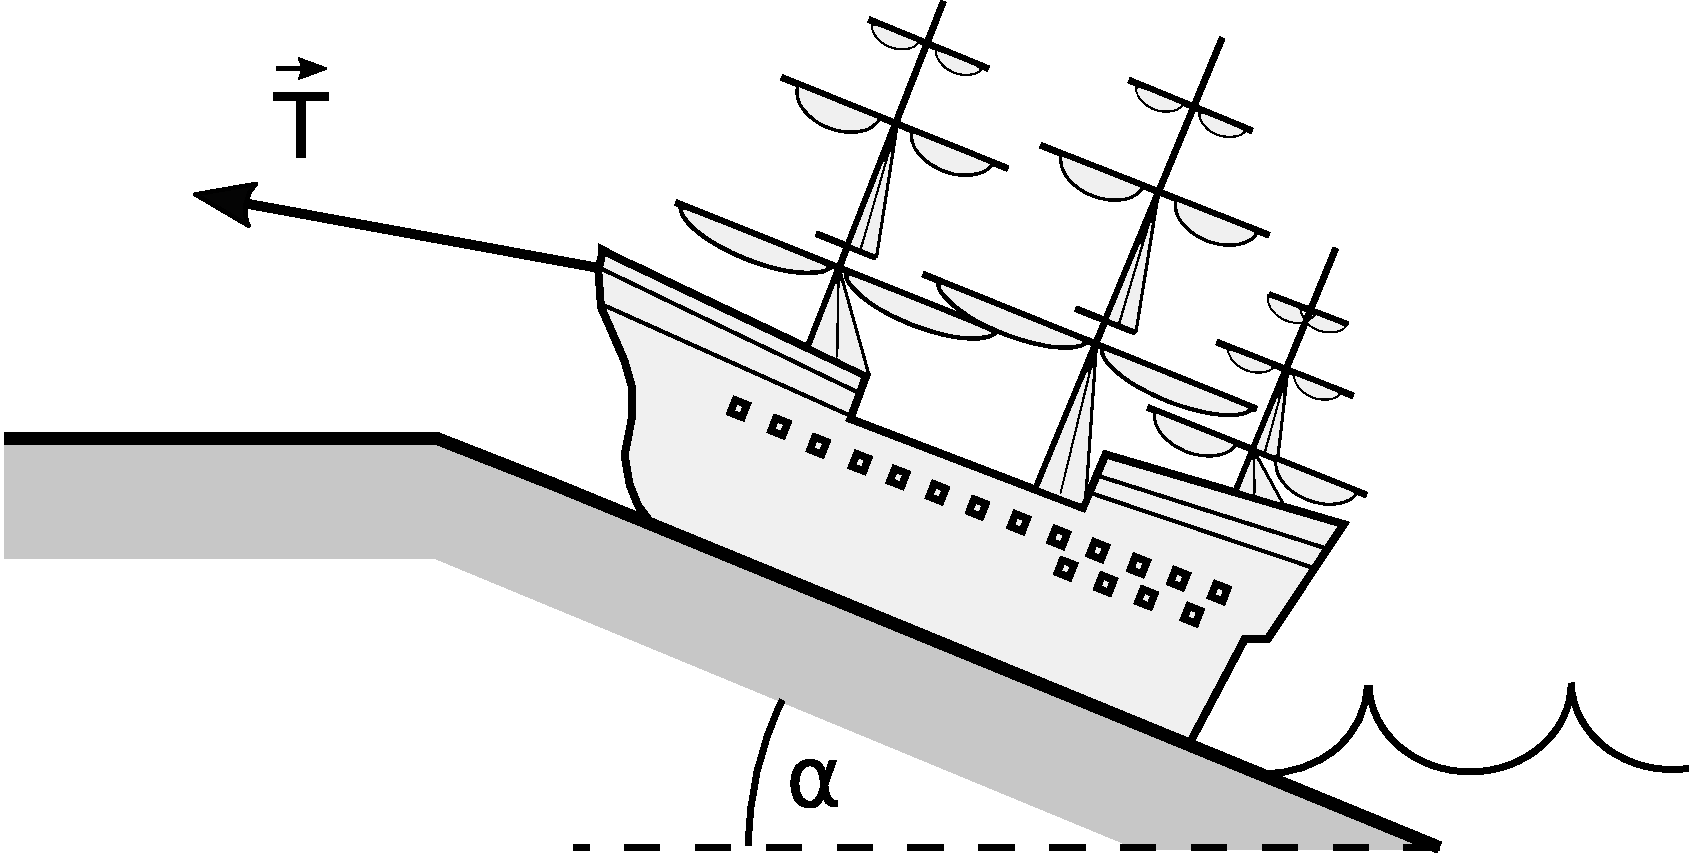
\includegraphics[width=0.4\linewidth]{2021-v2g-10-yl.pdf}
\end{center}


\hint

\solu
\textbf{Lahendus 1.} \\
Laevale mõjuvad raskusjõud $m\overrightarrow{g}$, kaldpinna toereaktsioon $\overrightarrow{N}$, hõõrdejõud $\overrightarrow{F}_h$ ja köie tõmbejõud $\overrightarrow{T}$. Et laev paigal püsiks, peab nende jõudude vektorsumma võrduma nulliga. Raskusjõud $m\overrightarrow{g}$ on konstantne suurus. Köie tõmbe kaldpinnaga ristuv komponent võib toereaktsiooni suurendada või vähendada ja vastavalt seosele $F_h=\mu N$ suureneb või väheneb samas proportsioonis ka hõõrdejõud. See tähendab, et vektori $\overrightarrow{N}+\overrightarrow{F}_h$ siht ei sõltu köie tõmbest $\overrightarrow{T}$, sest $\tan\gamma=F_h/N=\mu=\textit{const}$.

\begin{figure}[h]
\vspace{-0.0cm}
  \begin{center}
    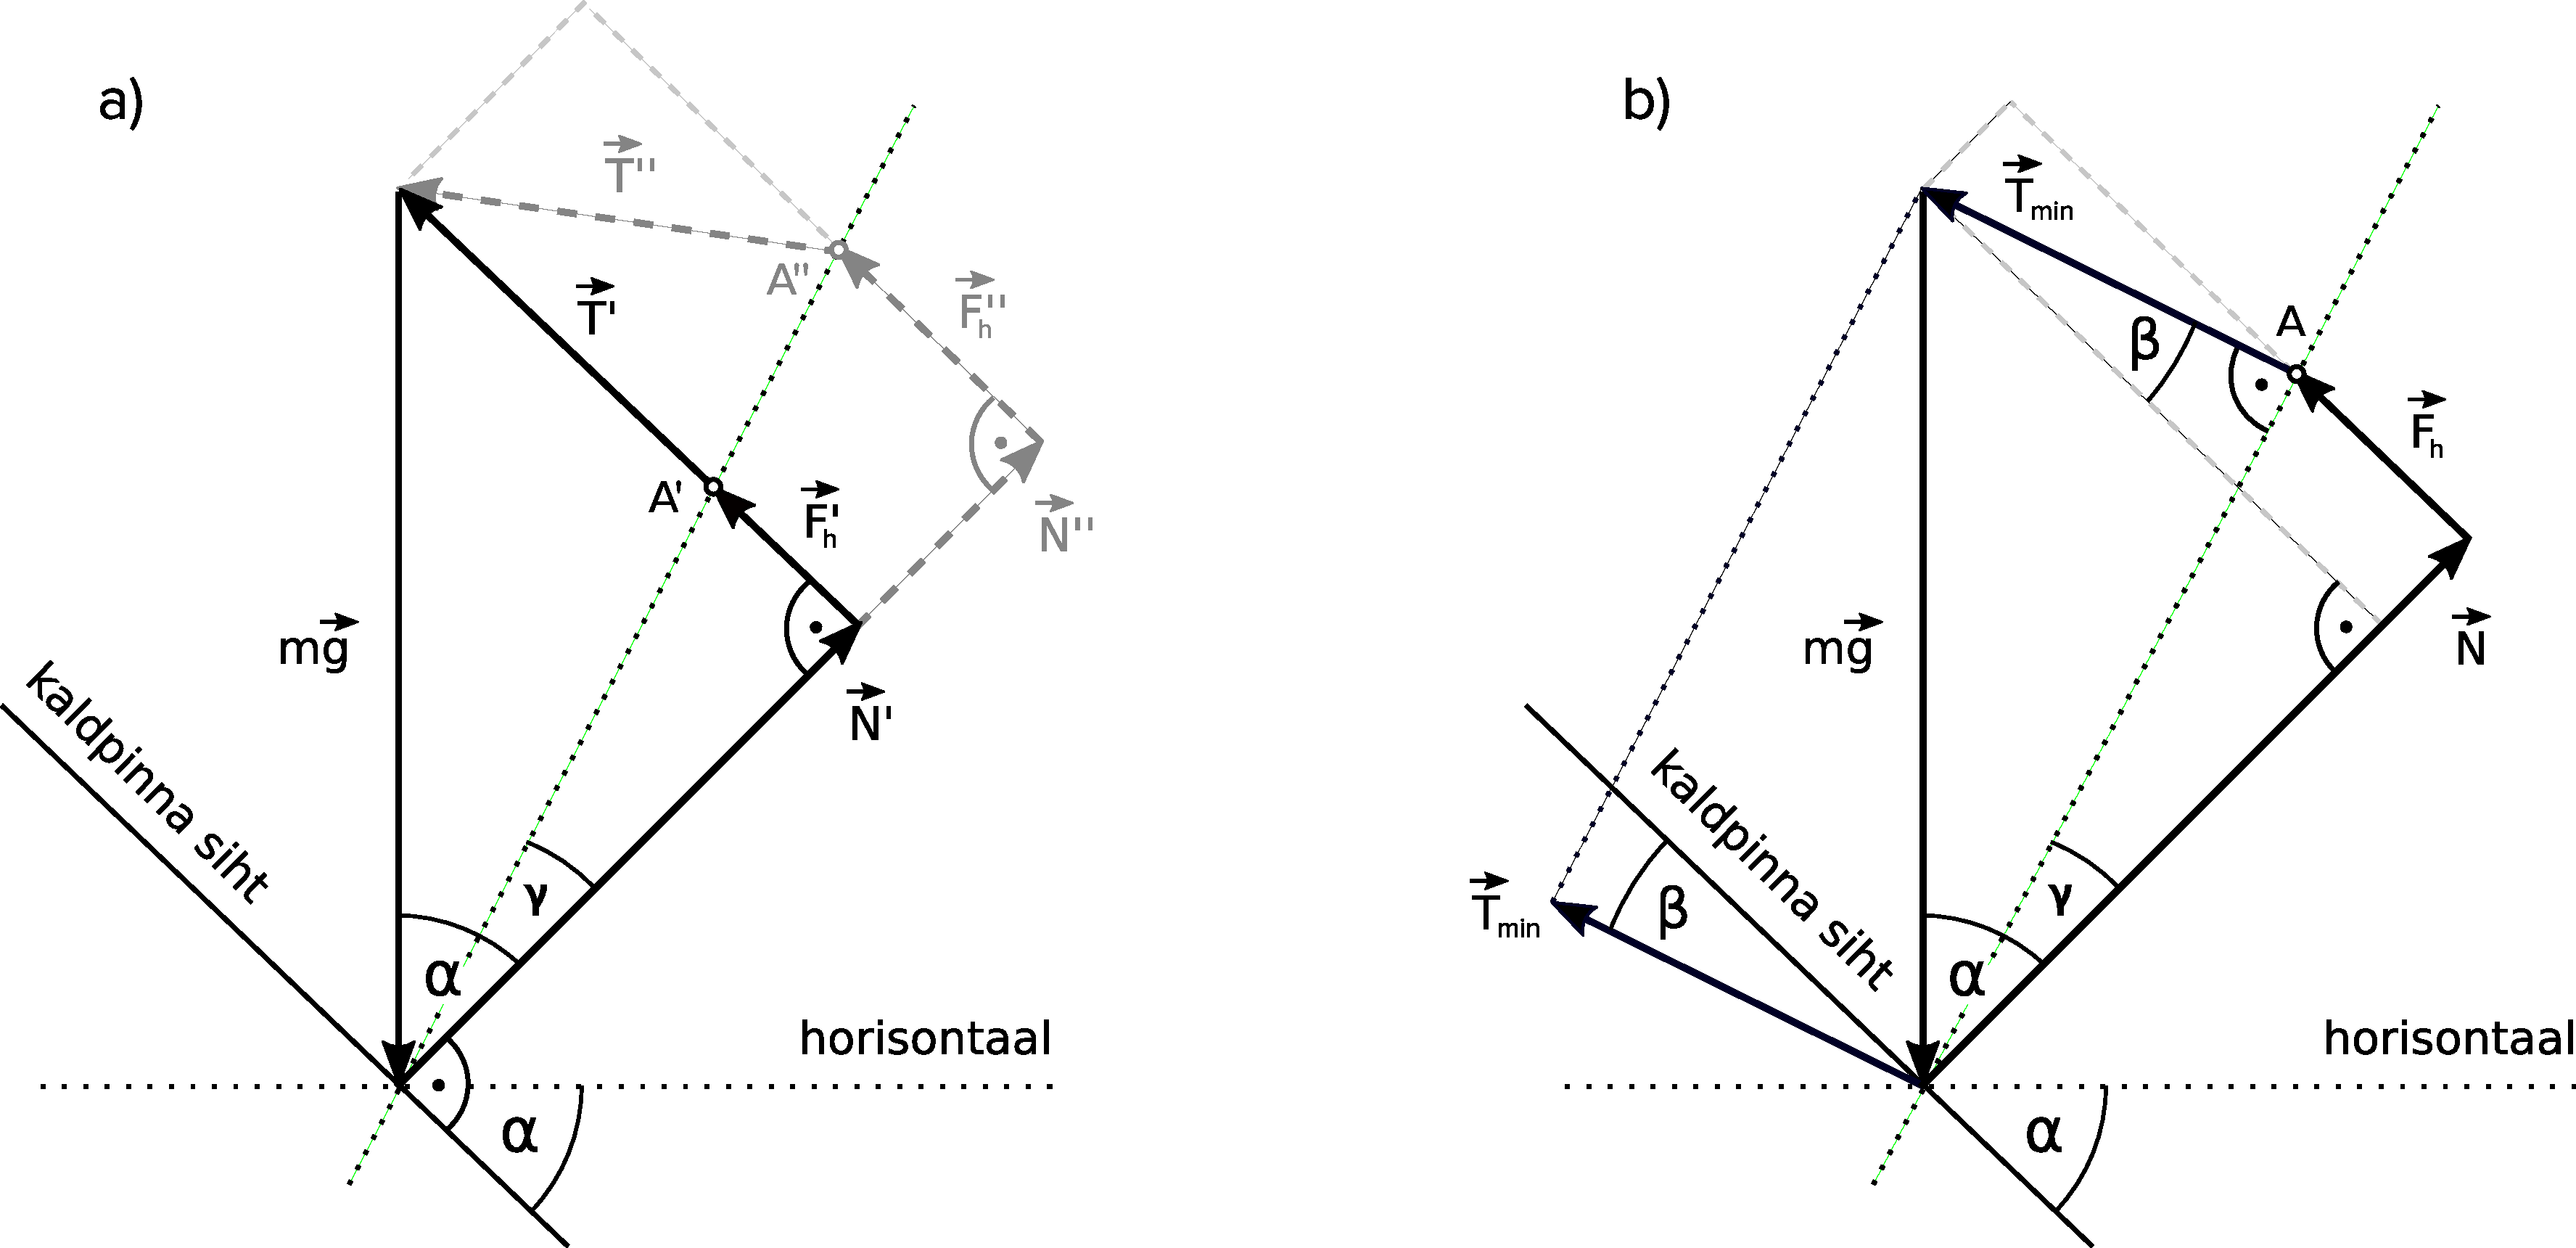
\includegraphics[width=0.9\linewidth]{2021-v2g-10-sol1.pdf}
    %\caption{}
  \end{center}
  \vspace{-0.5cm}
\end{figure}

Vaatleme kõigepealt olukorda, kus köie tõmbejõud mõjub paralleelselt kaldpinnaga. Joonisel a) on sellele olukorrale vastavad jõud tähistatud primmiga. Nüüd on lihtne näha, et võimalikele tasakaaluolekutele vastavad vektordiagrammid saame, kui liigutame punkti A suvaliselt vektoriga $\overrightarrow{N}+\overrightarrow{F}_h$ määratud sihis. Sealjuures paneme tähele, et vektori $\overrightarrow{T}$ pikkus on minimaalne siis, kui see asetseb $\overrightarrow{N}+\overrightarrow{F}_h$ sihiga risti. Selline olukord on kujutatud joonisel b). Sarnaste kolmnurkade võrdlemine annab minimaalsele tõmbele vastava nurga $\beta$ väärtuseks $\beta=\gamma=\arctan\mu$. Samalt vektordiagrammilt saame ka minimaalse tõmbe
\[T_{min}=mg\sin(\alpha-\gamma)=\]
\[=mg\sin(\alpha-\arctan\mu)= mg\frac{\sin\alpha-\mu\cos\alpha}{\sqrt{1+\mu^2}}.\]


\emph{Märkus:} Kui lahendaja eeldab ekslikult, et $\overrightarrow{T}_{min}$ on paralleelne kaldpinnaga ja tuletab sellest lähtuvalt lõppvalemi $T$ jaoks, siis hinnata lahendust
maksimaalselt 4 p. vääriliseks.

\begin{wrapfigure}{r}{0.5\textwidth}
\vspace{-0.5cm}
  \begin{center}
    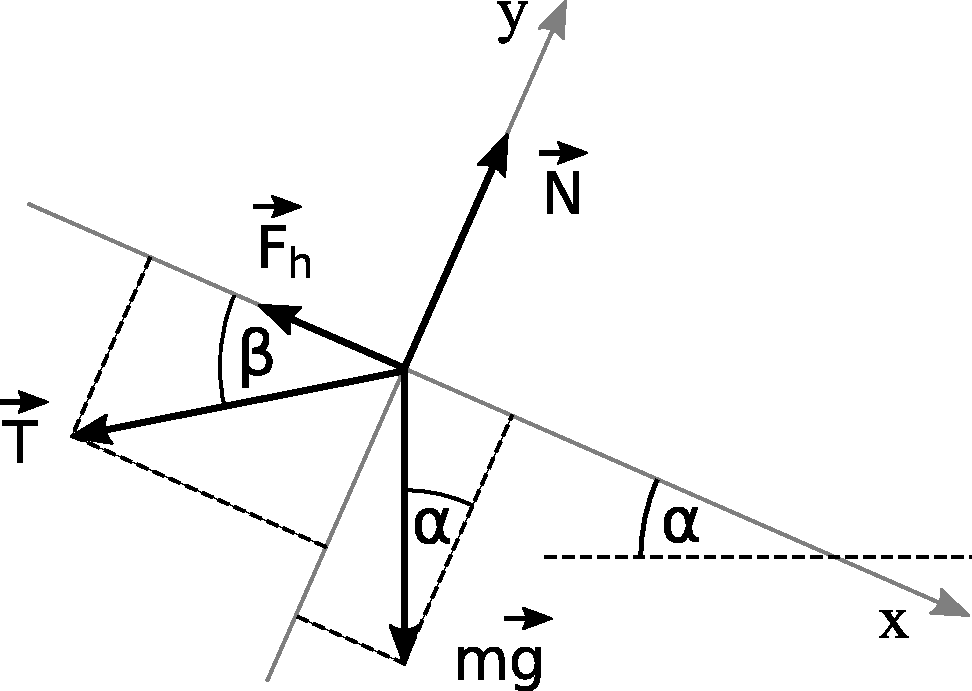
\includegraphics[width=0.8\linewidth]{2021-v2g-10-sol2.pdf}
  \end{center}
  \vspace{-0.5cm}
\end{wrapfigure}
\textbf{Lahendus 2.} \\
Olgu $\beta$ nurk kaldpinna sihi ja tõmbe $T$ sihi vahel. Valime ristkoordinaadistiku selliselt, et $x$-telg asetseb kaldpinna sihis. Kirjutame mõlema koordinaatelje jaoks välja jõudude tasakaalutingimused:
\begin{align*}
  F_x &= mg\sin{\alpha}-T\cos\beta-F_h=0,\\
  F_y &= N-T\sin\beta-mg\cos\alpha=0.
\end{align*}
Teisest võrrandist saame $N=T\sin\beta+mg\cos\alpha$
ja et $F_h =\mu N$, siis asendades need seosed esimesse võrrandisse saame
\[mg\sin\alpha-T\cos\beta-\mu T\sin\beta - \mu mg\cos\alpha=0,\]
millest
\[T=mg\frac{\sin\alpha-\mu\cos\alpha}{\cos\beta+\mu\sin\beta}.\]
Viimane valem annab tasakaalustava tõmbe $T$ suvalise nurga $\beta$ korral, kõik ülejäänud valemis esinevad parameetrid on ülesande tekstis fikseeritud suurused ehk konstandid.
Järelikult võime tõmmet $T$ vaadelda funktsioonina ühest muutujast $\beta$, st $T=T(\beta)$. Edasine ülesanne seisneb selle funktsiooni miinimumi leidmises. On selge, et $T$ on minimaalne siis,
kui nimetajas olev avaldis $\cos\beta+\mu\sin\beta$ on maksimaalne. Maksimumi määramiseks leiame selle avaldise tuletise $\beta$ järgi ja võrdsustame selle nulliga:
\[(\cos\beta+\mu\sin\beta)'=-\sin\beta+\mu\cos\beta=0, \]
millest $\mu=\tan\beta$ ehk $\beta=\arctan\mu$, mis ongi $T$ minimaalsele väärtusele vastav nurk. Asendades selle $T$ avaldisse saame
\[T_{min}=mg\frac{\sin\alpha-\mu\cos\alpha}{\cos(\arctan\mu)+\mu\sin(\arctan\mu)}= mg\frac{\sin\alpha-\mu\cos\alpha}{\sqrt{1+\mu^2}}.\]

\textbf{Hindamisskeem lahendusele 2.} \\
Õiged jõudude tasakaaluvõrrandid õpilase valitud koordinaatsüsteemis koos seletustega või joonisega, kus on näidatud võrranditele vastavad jõud ja nurgad [\textbf{4 p.}]\\
Korrektselt leitud $T$ üldavaldis [\textbf{2 p.}]\\
On aru saadud, et ülesanne taandub funktsiooni $T$ miinimumi leidmisele, ning et selleks tuleb kasutada tuletist. [\textbf{1 p.}]\\
Õigesti leitud tuletis ja sellest saadud miinimumile vastav seos $\mu=\tan\beta$, kus $\beta$ on nurk kaldpinna ja $\overrightarrow{T}_{min}$ vahel [\textbf{3 p.}]\\
Saadud õige lõppavaldis $T_{min}=mg\frac{\sin\alpha-\mu\cos\alpha}{\cos(\arctan\mu)+\mu\sin(\arctan\mu)}$ või sellega ekvivalentne avaldis, mis sisaldab ainult ülesande tekstis antud parameetreid
ja gravitatsioonikiirendust $g$ [\textbf{2 p.}]

\emph{Märkus:} Kui lahendaja eeldab ekslikult, et $\overrightarrow{T}_{min}$ on paralleelne kaldpinnaga ja tuletab sellest lähtuvalt lõppvalemi $T$ jaoks, siis hinnata lahendust
maksimaalselt 4 p. vääriliseks.
\probend